%\documentclass[prodmode]{acmsmall-ec16}
%\documentclass[prodmode,license]{acmsmall-ec16}
\documentclass[prodmode,permissions]{acmsmall-ec16}

% Package to generate and customize Algorithm as per ACM style
\usepackage[ruled]{algorithm2e}
\renewcommand{\algorithmcfname}{ALGORITHM}
\usepackage{amsmath,amsfonts,amssymb,bbm} 
\usepackage[numbers,sort&compress]{natbib} % for citet
\SetArgSty{textrm}  % for algorithm2e
\SetAlFnt{\small}
\SetAlCapFnt{\small}
\SetAlCapNameFnt{\small}
\SetAlCapHSkip{0pt}
\IncMargin{-\parindent}

%\conferenceinfo{EC'16,}{July 24--28, 2016, Maastricht, The Netherlands.}
%\CopyrightYear{2016}
%\crdata{978-1-4503-3936-0/16/07}
%\copyrighttext{Copyright is held by the owner/author(s). Publication rights licensed to ACM.}

\doi{XXXXXXX.XXXXXXX}% TeXSupport

\newcommand{\beq}{\begin{eqnarray}}
\newcommand{\eeq}{\end{eqnarray}}
\DeclareMathOperator{\wbf}{wBF}

% Document starts
\begin{document}

% Page heads
%\markboth{G. Zhou et al.}{A Multifrequency MAC Specially Designed for WSN Applications}

% Title portion
\title{
Attack-Tolerance in Structured Networks via Multipath Routing
\\ Draft: 2016-02-18
}
\author{EDWARD L. PLATT
\affil{University of Michigan}
DANIEL M. ROMERO
\affil{University of Michigan}}

\begin{abstract}
TODO
\end{abstract}

%ACM is moving forward with the 2012 Classification system: http://dl.acm.org/ccs_flat.cfm. Please generate the CCSXML tex code through the online interactive system and insert the code below. 

\begin{CCSXML}
<ccs2012>
</ccs2012>  
\end{CCSXML}

\ccsdesc[500]{TODO~TODO}

%\terms{Design, Algorithms, Performance}

\keywords{
censorship,
decentralization,
fault tolerance,
multipath,
networks,
peer-to-peer,
trust
}

\begin{bottomstuff}
This work is supported by TODO.

Author�s addresses: E.L. Platt and D.M. Romero, School of Information; email: \{elplatt,drom\}@umich.edu.
\end{bottomstuff}

\maketitle

TODO: Fix bibtex encoding. 

\section{Introduction}

Communication networks, expemplified by the Internet,
have become ubiquitous and critical infrastructural for
communities, organizations, and markets.
As with any critical infrastructure, the cost of a failure can be
immense, so methods for tolerating various kind of faults are an
important and ongoing area of research.
The key question is: what are the techniques and network structures that can
be used to create robust, fault-tolerant systems?

Many complex networks, including the Internet and World-Wide Web, exhibit
scale-free structure
\cite{barabasi_emergence_1999,barabasi_scale-free_2009}.
While scale-free networks tolerate random faults well,
they are highly susceptible to adversarial faults, i.e. attacks
\cite{albert_error_2000}.
For example, in 2008, YouTube suffered a worldwide outage for several hours
when a service provider in Pakistan advertised false routing information
\cite{hunter_pakistan_2008}.
The action (known as a {\em black hole attack}) was intended to censor YouTube
within Pakistan only, but resulted in a worldwide cascading failure.
Such vulnerabilities are not limited to any one system or protocol, but an
attribute of complex communication networks themselves.
General techniques for understanding and mitigating these vulnerabilities are
needed.

We consider a setting in which a source node in a network attempts to route information
to a target node by forwarding it through the edges of the network. We 
assume that some nodes in the network may be compromised by an attacker 
and will forward the wrong information to their neighbors. We assume 
a weak form of trust transitivity, where the source and the target are able to 
detect any compromised nodes that are a few hops away from them in the network.

Given this framework, we develop a \emph{multipath routing} technique to reduce 
the likelihood that compromised nodes are undetected during the information 
routing process by allowing multiple copies of a message to be sent through independent paths,
which can be used for error-detection and error-correction by the receiver. 

The multipath routing technique relies on the existence and detectability of
multiple independent paths between the source and the destination. Thus, network 
structure and routing algorithms play a key role in the success of the technique. We formally evaluate the 
effects of network structure on attack-resistance and show that the probability of undetected 
errors decreases exponentially with the number of independent paths between 
source and destination. Focusing on {\em structured networks}, in which links between nodes are 
constrained to a particular architecture, we propose an efficient multipath routing algorithm on an popular network
architecture, which is currently used for several applications -- the butterfly network \cite{}. 

Our main contributions are:
\begin{itemize}
\item{We present a formal {\em partial trust model},
which makes weaker transitivity assumptions than previous web-of-trust models,
and use this model to quantify the effects of network structure on
fault tolerance;}
\item{We show that the probability of successfully detecting an
adversarial fault increases exponentially with the number of disjoint untrusted
paths between the neighborhoods of the sender and receiver, and that this
value depends on network structure;}
\item{We present a scalable, efficient, and attack-tolerant multipath
routing algorithm on the butterfly network topology.}
\end{itemize}

Paper organization. TODO

\section{Background and Related Work}

In {\em structured networks}, link structure is predetermined.
Such networks can be designed to have favorable structural and routing properties,
at the expense of complicating the addition or removal of nodes.
Structured networks have been a popular tool in parallel and distributed
computing architectures \cite{kshemkalyani_distributed_2008}.
More recently, peer-to-peer systems based on distributed hash tables have used
structured ``overlay'' networks to map table keys to local TCP/IP routes
\cite{lua_survey_2005}.

Many distributed consensus protocols (such as those used by crypto-currencies)
are designed to provide tolerance against arbitrary or adversarial faults.
Byzantine agreement protocols
\cite{lamport_byzantine_1982,castro_practical_1999}
provide tolerance against arbitrary faults (including attacks) under
some circumstances, but are limited to small networks due to poor scalability.
Proof-of-work \cite{dwork_pricing_1993,nakamoto_bitcoin:_2008}
and proof-of-stake \cite{king_ppcoin:_2012}
provide better scalability, but wasteful of computational and energy
resources.
Federated Byzantine Agreement (FBA) \cite{mazieres_stellar_2015}
is scalable and optimal, guaranteeing that the protocol only fails when
success is impossible, although it does not provide a way to evaluate
the probability of failure.
All of these protocols rely on the assumption that their cryptography
cannot be compromised.
While cryptography can be extremely resistant to technological attacks,
it can still be compromised through coercion (e.g., legal action).
In additon, the fault-tolerance of FBA depends on redundancy in the network structure
but leaves an unanswerd question: how should a network be structured to achieve
fault tolerance?
This paper addresses both of these issues by analyzing the role of network
structure on adversarial faults, without relying on assumptions of cryptographic
integrity.

{\em Multipath} routing uses multiple paths when routing a message through a
network, in contrsast to traditional {\em unipath} routing, which uses
a single path.
Multipath routing can have many benefits, including reduced congestion,
increased throughput, and more reliability
\cite{qadir_exploiting_2015}.
Many of these routing protocols offer better security 
\cite{zin_survey_2015}.
Some approaches utilize redundant paths as backups for increased
fault tolerance
\cite{alrajeh_secure_2013},
and some specificially protect against adversarial faults
\cite{kohno_improvement_2012, khalil_unmask:_2010, lou_h-spread:_2006}.
The method of Liu et al.
\cite{liu_secure_2012}
routes multiple messages first to random peers and then
to their final destination.
The butterfly algorithm we present takes a conceptually similar approach.
Most work on multipath routing has been motivated by applications related to
wireless sensor networks (WSNs),
and have thus focused on ad-hoc, unstructured networks, often having a central
base station.
The trust model presented in this paper provides a more general way to evaluate
the effect of network structure on adversarial fault-tolerance.

\section{Attack-Tolerant Networks Infrastructure}

In this section, we describe the functional proprties required of an
attack-tolerant network infrastructure and how those properties translate
into constraints on network structure.
We pay special attention to a property we call
{\em stabilizing asymmetry}.

\subsection{Functional Properties}

In most cases, infrastructure must remain functional as it grows;
it must be {\em scalable}.
Systems having single points of failure are less tolerant against faults at those
points, which both raises the likelihood of a failure and creates targets
where attackers might be able to focus their resources efficiently.
Attack-tolerant infrastructure must minimize single points of failure;
it must be {\em decentralized}.
In some, but not all, cases it is also desirable that an infrastructure
provides {\em secrecy},
protecting the contents of a message or the identity of the sender.

We add one additional property, which we call {\em stabilizing asymmetry}.
In the context of international conflict,
\cite{mack_why_1975}
observed that power imbalance usually determines the outcome of a conflict
(with the more powerful side winning)
except in the special case of {\em asymmetric conflicts}.
In asymmetric conflicts, the same level of resource expenditure yields different
results for different parties.
There are two possible cases:
the attacker's resources are either more or less effective than the defender's.
We call the latter case stabilizing asymmetry,
because it lowers the incentive to attack.
With this in mind, an attack-resistant infrastructure will benefit from a high
level of stabilizing asymmetry.

\subsection{Structural Properties}

To achieve scalability, networks must be {\em sparse} and have a
{\em low diameter}.
In practical settings, humans and devices have an upper limit on the number
of connections they can maintain.
In sparse networks, the number of links grows slowly as the network grows in
size, allowing the network to scale without exceeding the nodes' capacity for
links.
Similarly, low-diameter guarantees that as a network grows, a short path will
still exist between any pair of nodes.
While low diameter guarantees a path exists,
paths are only useful if an efficient {\em routing} algorithm exists
to find them.

Redundancy in a network can help reduce single points of failure as well as
increase fault-tolerance.
One measure of redundancy is given by the ratio of edges to nodes
\cite{baran_distributed_1964}.
A single points of failure occur when a node holds a uniquely
central position,
and can be eliminated by adding alternative
paths around the node,
which increases the network's redundancy.
Similarly, redundancy in a network can enable fault-tolerance techniques
that reduce the effectiveness of attacks and creating stabilizing asymmetry.
When secrecy is desired, redundancy can help by allowing messages to be
divided into parts and sent along different paths so even if one path is
compromised, the whole message is not revealed.

Networks with {\em vertex transitivity} have the greatest protection agasint
single points of failure.
In vertex transitive networks, for any pair of nodes, an edge-preserving map
always exists from one node to the other.
In other words, all nodes occupy structurally indistinguishable positions
in the network.

\subsection{Trust}

The sparsity requirement has an important consequence for network infrastructure:
as a network grows, the number of nodes will exceed the number of links a given
node can support and many pairs of nodes will only be indirectly connected,
with all paths between them passing through at least one intermediary node.
These intermediary nodes are targets for potential attacks.
More specifically, the threat model is as follows: Alice sends a message to
Bob via one or more intermediaries, but some intermediaries may try to
either block or alter the message.
The ability to tolerate these types of adversarial attacks often depends on
Alice and Bob's ability to assume that some nodes have not been
compromised---to {\em trust} them.

Both centralized and decentralized approaches are commonly used to create
trust infrastructures.
Centralized approaches such as {\em public key infrastructure} (PKI)
suffer from a number of vulnerabilities
\cite{ellison_ten_2000},
which stem largely from the single points of failure inherent to
centralization.
Alternatively, the decentralized {\em web of trust} model
\cite{zimmermann_official_1995,ferguson_practical_2003}
allows individuals
to choose who they trust initially.
Trust is then extended to new individuals if they are vouched for by a
currently-trusted individual.
However, the web of trust approach assumes that trust can be extended
transitively,
which is not generally true
\cite{christianson_why_1997}.
We note that while such approaches are decentralized,
they do not incorporate redundancy and thus still suffer from single
points of failure.

\section{Partial Trust}

We now propose a decentralized trust model based on weaker transitivity
asumptions than existing web of trust models.
In following sections, we will use this model to utilize network redundancy and
minimize vulnerabilities due to single points of failure.
Our model is based on the assumption of partially-transitive trust.
While this assumption is still idealized, it is a more realistic improvement
on fully-transitive models.

Our model (Figure \ref{fig:trust-source})
is represented as an undirected graph or network,
with nodes representing individual
agents and edges representing direct and mutual trust relationships.
We define a {\em trust radius} $h$ and assume that trust is transitive
up to $h$ hops away.
In other words, the nodes $v$ trusts $w$ if the distance
$d(u,v) < h$.
We call the all such nodes the {\em trusted neighborhood} $T_h(v)$,
and all noes at exactly distance $h$ the {\em trust boundary} $B_h(v)$:
\beq
T_h(v) &=& \left\{ w \mid d(v,w) < h \right\} \\
B_h(v) &=& \left\{ w \mid d(v,w) = h \right\}.
\eeq
We assume that no nodes within the trusted neighborhood can be compromised
by an adversary of $v$.
However, by compromising all nodes in the trust boundary, an adversary can
ensure that all communications leaving the trusted neighborhood are compromised.

Source-to-network
\begin{figure}
\centerline{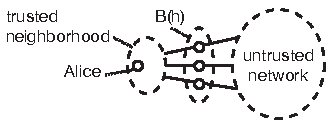
\includegraphics{fig-trust-source}}
\caption{
Illustration of the {\em partial trust} model.
Edges represent direct, mutual trust relationships.
Alice ($v$) trusts all nodes less than
$h$ hops away---her {\em trusted neighborhood} $T_h(v)$.
Beyond that, the nodes at distance $h$ form her {\em trust boundary} $B_h(v)$.
We assume adversaries are unable to compromise nodes in the trusted neighborhood.
By compromising all nodes in the trust boundary, an adversary can ensure that
all communications leaving Alice's trusted neighborhood are compromised.
}
\label{fig:trust-source}
\end{figure}

Now we consider a source $v$ (Alice) and a destination $w$ (Bob),
shown in Figure \ref{fig-trust-source-desitnation}.
We assume that a message beween Alice and Bob will not be compromised in
either of their trusted neighborhoods.
An adversary could compromise all possible paths between Alice and Bob
by compromising either Alice or Bob's entire trust boundary,
which requires compromising $\min(|T_h(v)|, |T_h(w)|)$ nodes.
In a vertex transitive network, these two trust boundaries will be the same size.
If disjoint paths exist connecting each node in Alice's trust boundary to
a node in Bob's, then the cut size between the two can never be smaller than
$|T_h(v)| = |T_h(v)|$,
so an adversary compromises fewer nodes, they cannot compromise all possible
paths between Alice and Bob.

\begin{figure}
\centerline{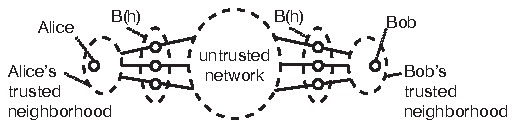
\includegraphics{fig-trust-source-destination}}
\caption{
Partial trust model with sender (Alice) and receiver (Bob).
If disjoint paths exist connecting each node in Alice's trust boundary to
a node in Bob's,
than an adversary needs to compromise at least $|T_h(v)|$ nodes to
compromise all possible paths between Alice and Bob.
}
\label{fig:trust-source-destionation}
\end{figure}

\section{Multipath Fault Tolerance}

Fault tolerance with partial trust and redundancy.

\subsection{Fault Tolerance}

Results

\begin{figure}
\centerline{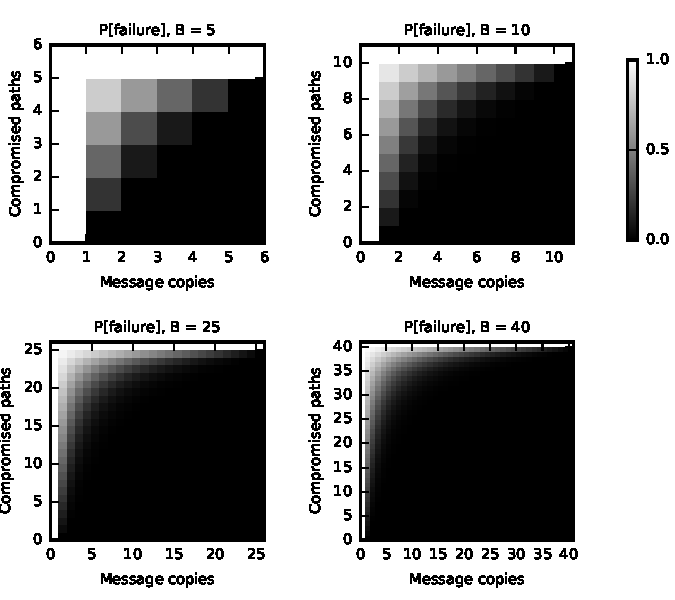
\includegraphics{fig-perror}}
\caption{TODO}
\label{fig:one}
\end{figure}

\section{Multipath Routing on the Butterfly Topology}

\subsection{Butterfly Network Topology}

We now describe a Concurrent Multipath Routing scheme on a specific family
of networks: the butterfly network \cite{}.
Several variations on the butterfly network exist.
Specifically, we utilize the wrap-around butterfly.
We denote the $m$-dimensional directed wrap-around butterfly as $\wbf(m)$:
\beq
\wbf(m) &=& (V, E_\downarrow \cup E_\rightarrow) \\
V &=& \mathbb{Z}_m \times \mathbb{Z}_{2^m} \\
E_\downarrow &=& \{((l,z),(l+1 (\text{mod } m),z) \nonumber \\
&& \; | \, l \in \mathbb{Z}_d, z \in \mathbb{Z}_{2^m}\} \\
E_\rightarrow &=& \{(l,z),(l+1 (\text{mod } m), z \oplus 2^l) \nonumber \\
&& \; | \, l \in \mathbb{Z}_d, z \in \mathbb{Z}_{2^m}\},
\eeq
where $\oplus$ represents the bitwise XOR operator.
Each node is associated with a level $l$ and an $m$-bit integer $z$.
There are two types of edges, shown in Figure \ref{fig:butterfly}.
Down edges ($E_\downarrow$) connect nodes sharing the same $z$ value
in a cycle of increasing level $l$.
Down-right edges ($E_\rightarrow$) also link to a node of level $l + 1$,
but one having the bitstring equal to $z$ with the $l$th bit flipped.

The wrap-around butterfly network has a number of properties making it useful for multipath routing:
\begin{description}
\item[Vertex transitivity]
The problem
of finding a route between arbitrary nodes $v$ and $w$
can be reduced to finding a route from node $(0,0)$ to some $\tilde{w}$.
\item[Logarithmic diameter]
For any two nodes, the length of the shortest path between them is logorithmic
in the size of the network.
\item[Constant degree]
In practical applications, each communication link requires additional resources,
such as physical infrastructure or entries in a routing table.
A constant degree limits the number of such resources needed as the network
grows in size.
\end{description}

\begin{figure}
\begin{center}
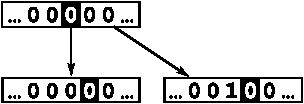
\includegraphics{fig-butterfly.pdf}
\end{center}
\caption{
Schematic illustration of the two types of edges in a directed butterfly network.
The node $(l,z)$ is shown as the bit string $z$ with a square around the $l$th bit.
\label{fig:butterfly}
}
\end{figure}

\subsection{Routing Algorithm: Overview}

This section gives an informal overview of the multipath routing algorithm.
In a wraparound butterfly network with trusted radius $h$,
the algorithm constructs $2^h$ disjoint paths between the trusted neighborhoods
of any two nodes, each parameterized by an $h$-bit string $s$
(see Table \ref{tab:routing}).
Each path cycles around the levels of the butterfly network (about) twice.
During the first cycle, the place-within-level $z$ of all nodes is set such that
no two paths overlap outside the trusted neighborhoods.
During the second cycle, the place-within-level is set to its destination value
and the algorithm terminates when the destination level is reached.

\begin{table}%
\tbl{Butterfly Multipath Routing Variables\label{tab:routing}}
{
\begin{tabular}{|l|l|}
\hline
NAME & VARIABLE \\\hline
butterfly dimension & $m \in \mathbb{Z}_+$ \\\hline
node level & $l \in \mathbb{Z} : 0 \leq l < m$ \\\hline
node place within level & $z \in \mathbb \{0,1\}^m$ \\\hline
trust radius & $h \in \mathbb{Z} : 1 \leq h \leq \lfloor m/2 \rfloor$ \\\hline
path index & $s \in \{0,1\}^h$ \\\hline
\end{tabular}
}
\end{table}%

\subsection{Routing Algorithm: Proof}

We now describe a routing scheme that provides $2^h$ redundant paths between
the $h$-hop trusted neighborhoods of any two nodes in an $m$-bit
wrap-around butterfly network.
Utilizing vertex transitivity, we label the source node as $(0, 0)$ and
denote the destination node as $w = (l_w, z_w)$.

Let $s$ be an integer such that $0 \leq s < 2^h$.
Let $v_s^{(t)} = (l^{(t)}, z^{(t)})$ be the $t$th node in the path labeled by $s$.
For convenience, we will omit the subscript $s$.
We define two partitionings of the integers in $\mathbb{Z}_{2^m}$:
one having the lowest $h$ bits matching the
bits of $s$, and one having the $h$ bits preceeding the destination level $l_w$
matching $s$:
\beq
S_s &=& \{z \in \mathbb{Z}_{2^m} | \forall i \in \mathbb{Z}_h z_i = s_i \} \\
R_s &=& \{z \in \mathbb{Z}_{2^m} | \forall i \in \mathbb{Z}_h z_{(l_w - h + i)} = s_i \}.
\eeq
Note that if $r \neq s$, then $S_s \cap S_r = R_s \cap R_r = \emptyset$.

We now construct a path such that between trusted neighborhoods $z^{(t)}$ is always
in $S_s$, $R_s$, or both, guaranteeing that the path does not overlap with the
other paths $v_r^{(t)}$.
Routing proceeds in stages, with the level $l$ increasing by 1 at each hop.
In Stage 1 ($0 \leq t < h$), down or down-right edges
are chosen such that the $t$th bit of $z^{(t+1)}$ is equal to the $t$th bit
of $s$. Throughout Stage 1, all nodes are within the sender's trusted neighborhood.
At the end of Stage 1, $z^{(h)} \in S_s$, and $z^{(t)}$ will remain so until the level loops
back to $0$ at $t = m$.

In Stage 2 ($h \leq t < l_w - h$), edges are chosen to make the $t$th bit of
$z^{(t+1)}$ match the $t$th bit of $z_w$.

In Stage 3 ($l_w - h \leq t < l_w$), the bits of $z^{(t)}$ are chosen to match $s$,
such that after the stage is complete, $z^{(l_w)} \in R_s$.

In Stage 4 ($l_w \leq t < m$), as in stage 2,
paths are chosen such that the $t$th bit of $z^{(t+1)}$ matches $z_w$.
After Stage 4, all bits of $z^{(m)}$ are equal to those of $z_w$
except for the first $h$ and the $h$ preceeding index $l_w$.
$z^{(m)}$ is also in both $S_s$ and $R_s$.

At this point, we define $\tau = t - m$.
In Stage 5 ($0 \leq \tau < h$), the first $h$ bits of $z^{(t)}$ are set to
match $z_w$, potentially removing $z^{(t)}$ from $S_s$.

In Stage 6 ($h \leq \tau < l_w - h$), all down edges are chosen, incrementing
the level without any effect on $z^{(t)}$.
At the end of Stage 6, $z^{(m + l_w - h)}$ is still in $R_s$ and
$v^{(m + l_w - h)}$ is now within the trusted neighborhood of $w$.

In the seventh, and final stage ($l_w - h \leq \tau < l_w$), the $h$ bits of $z^{(t)}$
preceeding index $l_w$ are set to match $z_w$.
After this stage, $v^{(m + l_w)} = w$ and routing is complete.

\begin{figure}
\begin{center}
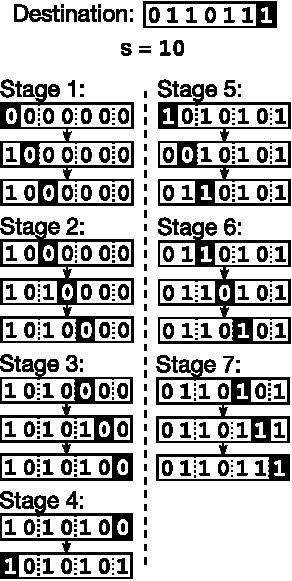
\includegraphics{fig-routing.pdf}
\end{center}
\caption{
\label{fig:routing}
}
\end{figure}

\section{Discussion}

Secrecy

Creation of the network.
Improves on web of trust.
Gives framework for determining where to build trust.

Applications
Distributed apps: storage, email, cryptocurrency, secure multiparty computation.
Wireless Sensor Networks

\section{Conclusion}

% Acknowledgments
\begin{acks}
The authors would like to thank TODO
\end{acks}

% Bibliography
\bibliographystyle{ACM-Reference-Format-Journals}
\bibliography{paper}

\end{document}
